\chapter{Analysis Software (ZeeD)}
\label{sec:ZeeD}
ZeeD (\Zee\ DESY) is a software solution, developed internally by the DESY ATLAS Standard Model group. It is based on the \Athena\ framework that is largely used in ATLAS, but uses it mostly for the input data reading, the AOD format, which is a standard for ATLAS. For performance reasons, the first step in the analysis is the conversion of the data to ZeeD internal format called TTrees (this is actually the name of the class in the ROOT framework used in this format, but in this section any mention of TTrees refers to ZeeD data format). This conversion allows for substantial speedup of the analysis, as well as to considerably reduce the space needed for the data storage.

The later stages of the analysis include the selection (application of cuts), reweighting (in case of MC sampes) and plotting. ZeeD also allows to apply the systematic shifts as well as use ToyMC for uncertainties propagation studies.

The structure of ZeeD can be seen in Figure~\ref{fig:zeed_flowchart}. During the analysis, \texttt{ZeeDLauncher} initializes the \Athena\ framework and provides all the configurations first. The framework gives access to the input data files and the configuration parameters. Then \texttt{ZeedAnalysisLoop} starts to iterate through the events in the input files. For each event it may run several iterations of the analysis, if the systematic study is required (one iteration for each systematic shift). In case of ToyMC systematic study (the systematic propagation technique that will be discussed in Section~\ref{sec:ZeeD_toymc}), the number of iterations can be as high as several hundred. Each iteration is contained within a separate \texttt{ZeeDAnalysisChain} which represents the conditions of the required systematic shift (including the "no shift" case). The actual corrections and possible systematic shifts is applied inside \texttt{ZeeDCalculator}, which also takes input from several external tools developed inside ATLAS. Corrected (and possibly shifted electrons are then passed to the various \texttt{ZeeDFinder}'s, which then try to construct all possible boson candidates from them. Every analysis has its own finder which only constructs the bosons that comply with the respective analysis criteria, e.g. \Zee\ central-central, \Zee\ central-forward or \Wenu. The bosons are then passed to the \texttt{ZeeDAnalysisCutSelector} which applies the set of cuts to each boson candidate. There are several selectors, one for each set of cuts that is used in any analysis, sometimes with several variations for different cross-checks. After all cuts are applied, the boson candidate passing the tightest selection is considered to be the best candidate, and if it also passes all the cuts mandatory for the analysis, it is passed to \texttt{ZeeDHistManager} to be included in the final results. In the following sections all these stages and subsystems of ZeeD will be described in details.

\begin{figure}
\center{
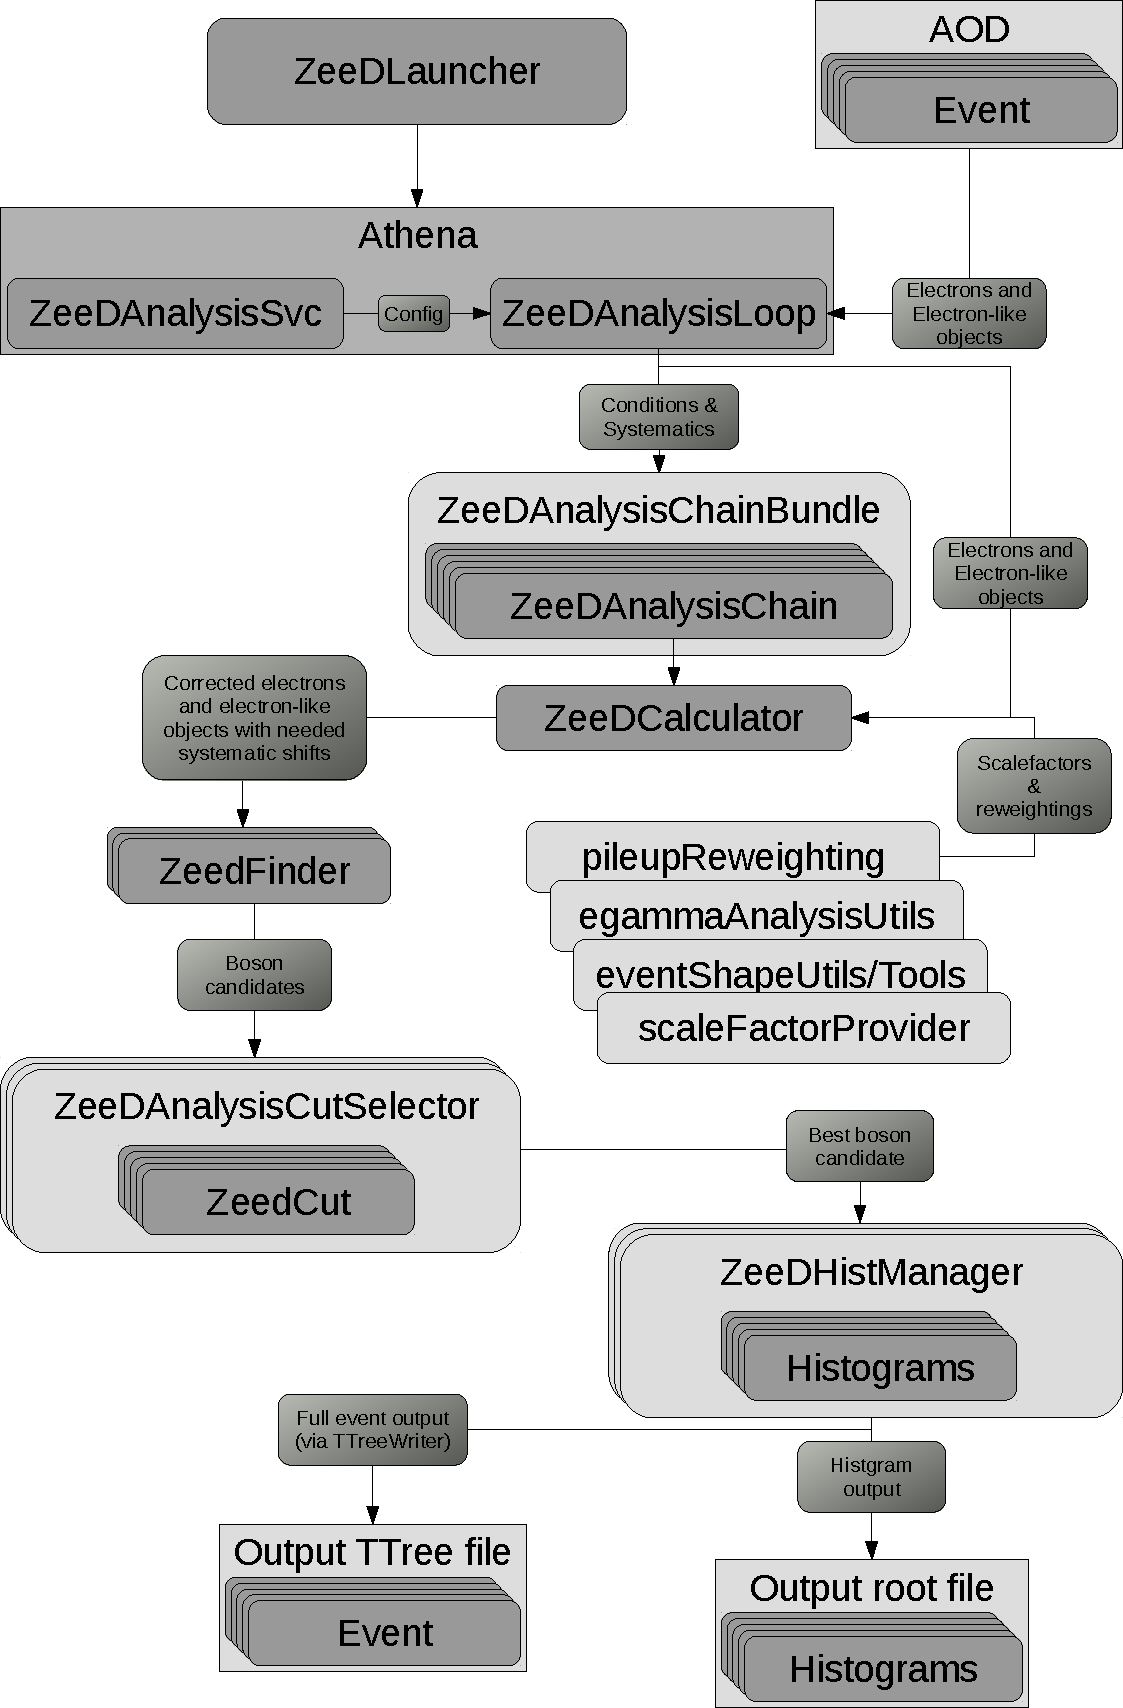
\includegraphics[width=0.8\textwidth]{figures/zeed_flowchart.pdf}
\caption{The functional flowchart of the ZeeD analysis software.}
\label{fig:zeed_flowchart}}
\end{figure}

\section{TTrees}
\label{sec:ZeeD_TTrees}

The data from the ATLAS detector comes in the form of the AOD files, which a special format based on the ROOT data file format and developed internally by the ATLAS. The format allows the seamless reading and writing of the various data objects (e.g. tracks, EM clusters, reconstructed particles, etc) within the \Athena\ framework. In AOD files all the information reconstructed from the collision is stored. In case of simulated events (i.e. MC) there is also the information about the generated particles, the so-called "truth particles", which can be used to determine the efficiency of the reconstruction algorithms and the analysis software.

Most of the information stored in the AODs is not used in the \Zee\ analysis, which only needs reconstructed electrons. And not even all the information available for the electrons is needed, as we only apply cuts and construct various differential cross-sections. During the analysis workflow, ZeeD uses about $0.1\%$ of all the information stored in the AODs, but because of the ATLAS framework structure, all the content of it should be read from the store and preloaded into the memory, which consumed most of the time needed for the analysis iteration. Also, because of the nature of the ATLAS data storages and the GRID farms used for the analysis, it was prone to errors, and it would require several attempts and consume much time to finish even one iteration.

The solution for this problem is to extract the needed information from the AOD files and store it in the simplified structure in ROOT ntuples. Similar solution was later used for the AOD successor - xAOD format. But whereas xAOD allows all this to be done automatically, for the 2011 the custom tool for manual conversion had been developed. The software chain for the TTree writing is the same as the analysis chain. The data is read from the AODs, the preselection cuts are applied to reduce the amount of data, and the output information is written out, which in this case is the raw events.

Because of this similarity, the same software - ZeeD - was used for the TTrees production as well. It is capable of reading data from AODs, it has all the cuts applicable for preselection, and it is capable of outputting any kind of data from the selected events. With the corresponding setup, the ZeeD workflow will be suitable for this production.

\section{Boson Finder}

The main target of all the analyses that are conducted using the ZeeD software are the Z bosons, so finding all the possible Z boson candidates in every event is always the first task. The ZeeD component that does that job is the boson finder class. On the basic level it just creates a boson candidate for every possible pair of electrons, but further in the analysis it keeps track of all the bosons and records all the intermediate results for each one. Ultimately, we won't accept more than one boson from any event, so every boson candidate is assigned a special "score" of how well it passes the various cuts: every passed cut adds one point to the boson's score, except for one cut that checks that the di-electron mass is very close to $M_Z$, which adds ten points. When there are several boson candidates that pass all the required cuts, the candidate with the highest score is picked for the final results. In case of the final \Zee\ analysis this situation is impossible, though, as we require not more than two suitable electrons. This mechanism is used for various tests and cross-checks.

\section{Cuts}

The analysis implications of different cuts will be discussed in the Section~\ref{sec:Sel_cuts}. Here we'll discuss the technical aspects of the event selection.

From the technical point of view, every cut is a restriction on one or several variables of the reconstructed event. Every event can pass or fail a given cut, and the infrastructure should be able not only to provide information whether some event passed all the cuts or not (which is the only thing that is important for the analysis itself), but also to show the results of all the cuts separately. This is called a "cut-flow" and it is used for debugging purposes and cross-checking. In the situation when different groups using different software come to different results for the same analysis, the ability to find out on which cut every particular event was filtered out is very helpful. With it we can find out which cut gives different results across different analysis groups.

The other functionality important for the cuts facility is the cut reversal which is useful for the background estimation. The background estimation methods (discussed later in Section~\ref{sec:Bkg}) require to select the events where electron pass some specific cuts, but fail some other specific cuts. To achieve that, the cuts framework construct the bit-mask for every event, where every bit corresponds to the cut, and displays whether that event passed or failed that cut. After the bit mask is composed, we can compare it to the desired bit-mask, and include or exclude the event from the analysis.

\section{Reweighting}

The reweighting of the MC events is used for the fine-tune of the simulation to the real data. The weights are calculated based on the well defined distributions in data (such as the trigger efficiencies) and bring the corresponding MC distributions in accordance with the data. The calculation of the weights is done using some well-measured process. For instance, \Zee\ decay is good for calculating the trigger efficiency, since it has a low background in the peak region, and has two electrons which allows the use of the tag and probe method. The calculation of the weights is thus done by conducting the same analysis on MC and real data without any corrections, and then comparing the distributions, for which we want to introduce reweighting. Weights are usually applied in bins, so the result of the weight calculation would be a histogram, sometimes two-dimensional, which would cover the kinematic plane for the variable being reweighted. Apart from the weight itself, the statistical and systematical uncertainties for every bin are also calculated, and stored in the similar histograms.

After the weights are calculated, they are used during the analysis. The weights are picked for every event based on its properties, and then the final weight of the event is calculated by multiplying all the weights from different corrections. This weight is later used during the histograms plotting. Since every weight comes with the statistical and systematical uncertainties, they also contribute to the calculation of the final error for the analysis. The process of calculation of the impact of different uncertainties to the final combined error would be discussed in the Section~\ref{sec:ZeeD_toymc}.

\section{Histogram managers}

The results of the analysis are the histograms, showing the various distributions of the physical quantities. The facilities responsible for that are the histogram managers. Each manager represents some aspect of the analysis, and creates and fills one or several histograms, which are thus grouped in it by their role. Each of the managers can be attached or detached during the launch setup, which allows to conduct various analyses with the same software, as long as this analysis deals with electrons, muons, and missing \et\ (the only kind of data that ZeeD extracts from the egamma data stream).

For the \Zee\ analysis the important managers would be an electron manager (plots the various distributions of the electrons properties, such as energy, \et, geometrical variables, etc), a ZCF manager (plots the properties of the central-forward Z-bosons), and (in case of MC samples) the truth managers (plots the truth information for the given event).

There is also one special histogram manager, which actually doesn't plot any histograms, but uses the same interfaces. It is the ZeeD TTree writer, which dumps out the content of the event in the ROOT tuples. This histogram manager is used to produce the TTrees that were previously discussed in Section~\ref{sec:ZeeD_TTrees}.

\section{Systematics and ToyMC}
\label{sec:ZeeD_toymc}

One of the most important aspects of the analysis is the uncertainty estimation. The uncertainties come in two forms: correlated and uncorrelated between bins. A statistical uncertainty is always considered to be uncorrelated, while the systematical uncertainty can be of both kind, as well as a mixture of them. Two methods of the uncertainty propagation exist: the offset method and the ToyMC method. The first method is usually employed in case of fully correlated uncertainties, and consists of calculating the results with all the source distributions shifted up or down by the amount of the corresponding uncertainty. The source distributions here are not only the data itself, but also all the scale factors and correction, which all come with their own uncertainties. Each uncertainty should be shifted separately and the shift in the produced result would amount to its propagated value.

The ToyMC method is more advanced as it allows to propagate both uncorrelated uncertainties, and the mixture of the correlated and uncorrelated ones in the form of so-called combined ToyMC. The method consists of producing of a high number of variations of the input data by the use of so-called biases, that are the Gaussian distributed shifts with the standard deviation equal to the value of the statistical and uncorrelated uncertainties
\begin{equation}
B^i = \Delta S_\mathrm{stat+uncor} \cdot \mathrm{Gauss}(0,1)\;\;\; i=0,...,N_\mathrm{toys}\,,
\end{equation}
where $B^i$ is a bias and $N_\mathrm{toys}$ is order of hundreds. In case of the combined ToyMC, all sources of the correlated errors also contribute to the bias
\begin{equation}
\left. B^i = \Delta S_\mathrm{stat+uncor} \cdot \mathrm{Gauss}(0,1) + \sum\limits_{s}S^k_{\mathrm{cor},s} \cdot \mathrm{Gauss}(0,1)\right\vert_k \;\;\; i=0,...,N_\mathrm{toys}\,,
\end{equation}
where $B^i$ as again a bias, and $s$ runs over all sources of the correlated uncertainties. The main difference in a treatment of the correlated and uncorrelated uncertainties is that the gauss value for $S_\mathrm{stat+uncor}$ is constant bin-wise, so the whole distribution is shifted uniformly, while an case of $S^k_{\mathrm{cor},s}$ every bin is treated independently, which is denoted by the index $k$ which runs over bins. The biases are then applied (added) to the input data to construct a set of $N$ inputs. After the unfolding procedure (see Sections~\ref{sec:ZCS_bbb_unf} and~\ref{sec:ZCS_bay_unf} for the description of the unfolding) this results in $N$ unfolded distributions. The distributions can then be fitted by gauss to find out the median value and an error, which would be the standard deviation of the fit, or alternatively, if the results of the analysis are intended to be used in a consequent ToyMC, then the distributions are combined into a covariance matrix in order to decompose it to nuisance parameters to find out the correlated and uncorrelated components of the unfolded uncertainties. More on the correlation studies can be read in~\cite{lib:elec_support}.

ZeeD software offers an easy way to conduct a ToyMC uncertainty propagation through the system of so-called "shelves" or "analysis chains", which is essentially a variation on the same analysis with different input parameters. With enabling the ToyMC method, ZeeD will create a large number of shelves (the default being 100) and automatically calculates the biases for every shelve by the use of the combined ToyMC method. The results for all the variations are then stored independently in the output file for future process.
